\documentclass[tikz,border=10pt]{standalone}
\usepackage{amsmath}
\usepackage{tikz}
\usetikzlibrary{arrows.meta, positioning}

\begin{document}
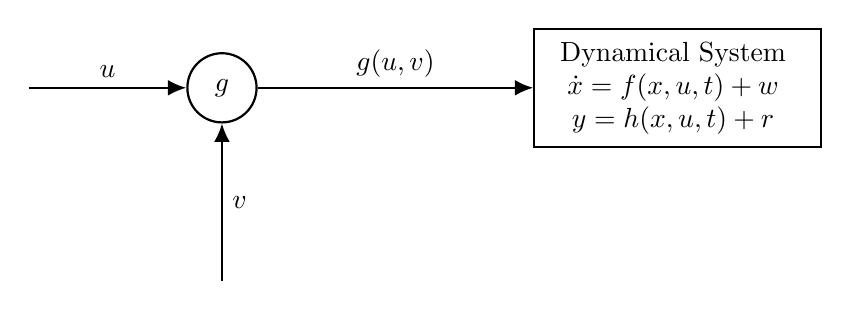
\begin{tikzpicture}[
    block/.style = {draw, thick, minimum height=2em, minimum width=4em, align=center},
    circ/.style = {draw, circle, thick, minimum size=2.5em, inner sep=0pt},
    arrow/.style = {thick, -{Latex[width=2mm]}},
    node distance=2cm and 2.5cm
  ]

  % Circle node g
  \node[circ] (g) {$g$};

  % System block to the right of g
  \node[block, right=3.5cm of g] (system) {
    \begin{tabular}{c}
      Dynamical System \\
      $\dot{x} = f(x,u,t) + w$ \\
      $y = h(x,u,t) + r$
    \end{tabular}
  };

  % Arrow u into center-left of g
  \draw[arrow] 
    ([xshift=-2cm]g.west) -- 
    (g.west) 
    node[midway, above] {$u$};

  % Arrow v from below into bottom of g
  \draw[arrow] 
    ([yshift=-2cm]g.south) -- 
    (g.south)
    node[midway, right] {$v$};

  % Arrow from g to system
  \draw[arrow] 
    (g.east) -- 
    (system.west) 
    node[midway, above] {$g(u,v)$};

\end{tikzpicture}
\end{document}
